%%%%%%%%%%%%%%%%%%%%%%%%%%%%%%%%%%%%%%%%%
% Beamer Presentation
% LaTeX Template
% Version 1.0 (10/11/12)
%
% This template has been downloaded from:
% http://www.LaTeXTemplates.com
%
% License:
% CC BY-NC-SA 3.0 (http://creativecommons.org/licenses/by-nc-sa/3.0/)
%
%%%%%%%%%%%%%%%%%%%%%%%%%%%%%%%%%%%%%%%%%

%----------------------------------------------------------------------------------------
%	PACKAGES AND THEMES
%----------------------------------------------------------------------------------------

\documentclass{beamer}

\mode<presentation> {
\usetheme{CambridgeUS}
\usecolortheme{rose}
}

\usepackage[utf8]{inputenc}
\usepackage[russian]{babel}
\usepackage{graphicx}
\usepackage{listings}
\usepackage{inconsolata}
\usepackage{amsmath}
\usepackage{amsfonts}
\usepackage{amssymb}
\usepackage{color}
\usepackage{tikz}
\usepackage{booktabs}

\usetikzlibrary{automata,positioning}
\usetikzlibrary{shadows}
\definecolor{bluekeywords}{rgb}{0.13,0.13,1}
\definecolor{greencomments}{rgb}{0,0.5,0}
\definecolor{redstrings}{rgb}{0.9,0,0}

\usepackage{listings}
\lstset{language=[Sharp]C,
    showspaces=false,
    showtabs=false,
    breaklines=true,
    showstringspaces=false,
    breakatwhitespace=true,
    escapeinside={(*@}{@*)},
    commentstyle=\color{greencomments},
    keywordstyle=\color{bluekeywords},
    stringstyle=\color{redstrings},
    basicstyle=\small\ttfamily,
    breaklines=true,
    tabsize=2,
}

\AtBeginSection[]{
    \begin{frame}
    \vfill
    \centering
    \begin{beamercolorbox}[sep=8pt,center,shadow=true,rounded=true]{title}
        \usebeamerfont{title}\insertsectionhead\par%
    \end{beamercolorbox}
    \vfill
    \end{frame}
}

%----------------------------------------------------------------------------------------
%	TITLE PAGE
%----------------------------------------------------------------------------------------

\title[DTW]{Динамическое выравнивание многомерных временных рядов}

\author{Моргачев Г., Смирнов В., Липницкая Т., \\ Руководитель: Гончаров А.}
\date{\today}

\begin{document}

%------------------------------------------------

\begin{frame}
\titlepage 
\end{frame}

%------------------------------------------------

\begin{frame}
\frametitle{Сравнения рядов}
	\begin{block}{Проблемы}
        \begin{itemize}
            \item Растяжение
            \item Сдвиги
        \end{itemize}
    \end{block}
    \begin{figure}
        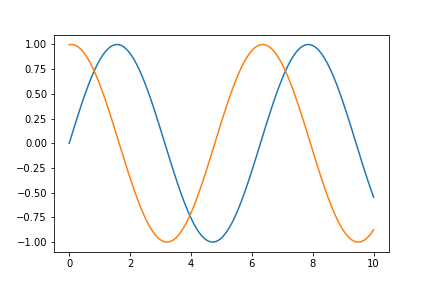
\includegraphics[width=0.6\linewidth]{2}
    \end{figure}
\end{frame}

%------------------------------------------------

\begin{frame}
\frametitle{DTW}
    \begin{block}{DTW}
        Выравнивание рядов друг относительно друга
    \end{block}
    \begin{figure}
        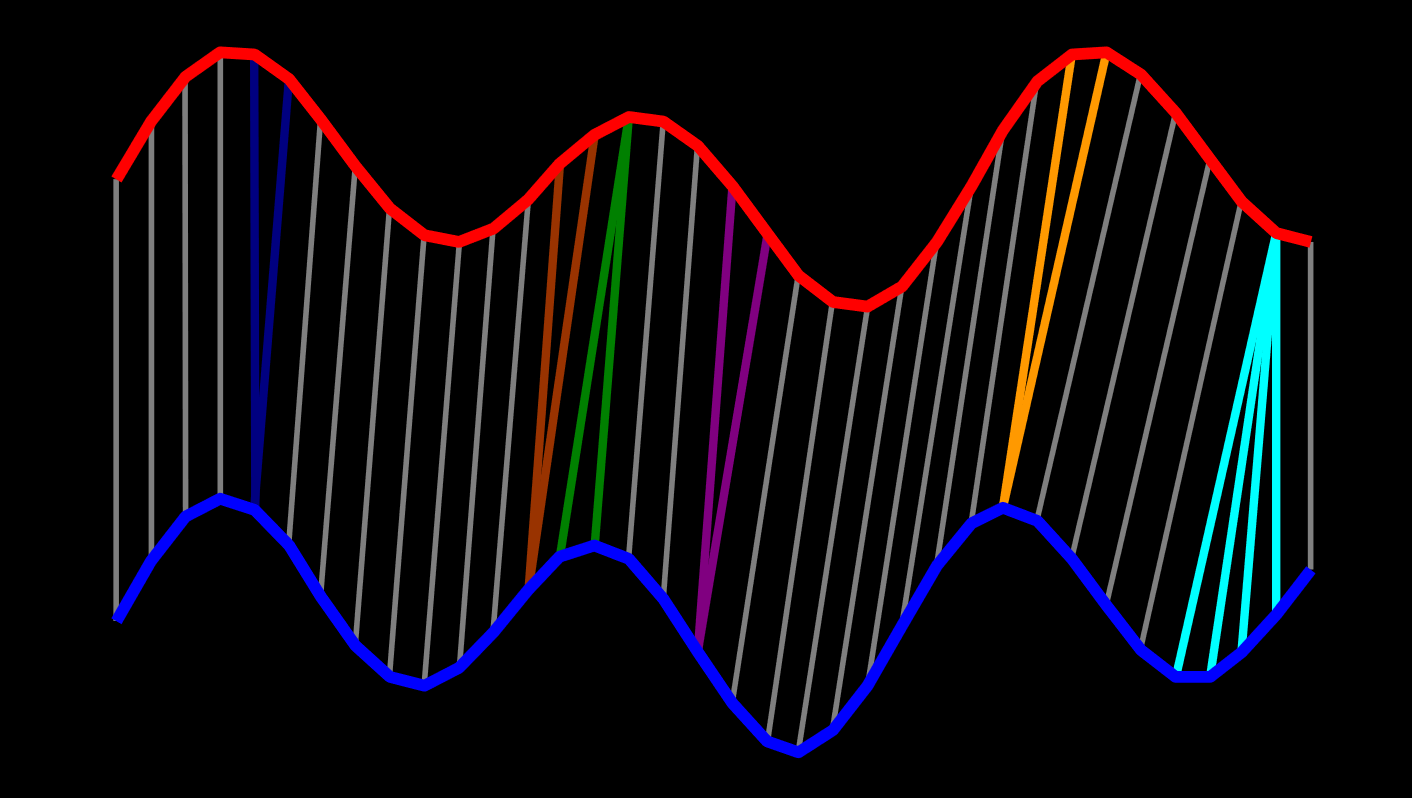
\includegraphics[width=0.6\linewidth]{1}
    \end{figure}
\end{frame}
    
%------------------------------------------------

\begin{frame}
\frametitle{Многомерная DTW}    
    \begin{block}{Особенность}
        Необходимость выбора функции расстояния между соответственными точками ряда
    \end{block}

    \begin{block}{Постановка задачи}
        Зависимость качества кластеризации временных рядов от выбора функции расстояния между ними
    \end{block}
\end{frame}
    
%------------------------------------------------

\begin{frame}
\frametitle{Задача}
    \begin{block}{}
        Множество временных рядов
        $\mathbb{S} \subset \mathbb{R}^{l \times n}$, где $l$ \-- количество каналов,\\ $n$ \-- длина ряда.

        $\forall s_i \in \mathbb{S}$ задано ${y_i \in \mathbb{Y}}$ \-- множество меток классов.

        Функции расстояния между векторами $\mathrm{R}$:
        $$
            \mathrm{R} = \{\rho: \mathbb{R}^n \times \mathbb{R}^n \rightarrow \mathbb{R}^+ \}
        $$

        Соответствующие \textbf{DTW}
        $$
            g_{\rho}: \mathbb{S} \times \mathbb{S} \rightarrow \mathbb{R}^+ 
        $$
    \end{block}
\end{frame}

\begin{frame}
    \frametitle{Задача}
    \begin{block}{}
        Пусть $ S \subset \mathbb{S}, \ \ |S| = N$ \-- выборка

        Матрица попарных расстояний:
        $$
            D(g_\rho(S)) = ||D_{ij}||, \ \ D_{ij} = g_\rho(s_i, s_j),\ \ s_i, s_j \in S 
        $$
        Кластеризатор:
        $$
            f: D \rightarrow Z^N, \ \text{Z \-- множество меток кластеров}
        $$

    \end{block}
\end{frame}

\begin{frame}
    \frametitle{Задача}
    \begin{block}{Функции качества}
    \begin{align*}
        Q_1(f(D), S) &= \frac{1}{|Z|}\sum\limits_{z \in Z} \max_y \frac{N_z^y}{N_z}  \\
        Q_2(f(D), S) &= \frac{1}{|Z|}\sum\limits_{z \in Z} \max_y \frac{(N_z^y)^2}{N_z N^y}
    \end{align*}
    \end{block}

    \begin{block}{Постановка задачи}
        $$
            Q_i(D(g_\rho(S), S) \rightarrow \max_{\rho}
        $$
    \end{block}
\end{frame}
    
%------------------------------------------------

\begin{frame}
    \frametitle{Эксперимент}
    \begin{block}{Кластеризация}
        \textbf{Иерархическая} с функциями расстояния между кластерами: 
        \begin{enumerate}
            \item \textit{complete:}  $d(A, B) = \max\limits_{a \in A, b \in B}(dist(a, b))$ 
            \item \textit{weighted:}  $d(A,B) = \dfrac{(dist(S,B) + dist(T,B))}{2}$, где кластер $A = S \cup T$
            \item \textit{weighted:}  $d(u,v) = \sum\limits_{a \in A, b \in B} \dfrac{d(a, b)}{(|A|*|B|)}$ 
        \end{enumerate} 
    \end{block}
\end{frame}
 
\begin{frame}
    \frametitle{Эксперимент}   
    \begin{block}{Данные}
        Размеченные данные ускорений акселерометра телефона
        \begin{itemize}
            \item 6 состояния человека
            \item 3 канала
            \item Разбиты на ряды по 50 точек
            \item Размер выборки - 2048
            \item Производится нормализация данных
        \end{itemize}
    \end{block}
\end{frame}
    
%------------------------------------------------

\begin{frame}
    \frametitle{Результаты}   
    \begin{center}
        \begin{table}
        \begin{tabular}{ll|rrr|rrr}  
            \toprule
            & & \multicolumn{3}{c|}{$Q_1$} & \multicolumn{3}{c}{$Q_2$} \\
            \cmidrule(r){3-8}
        $\rho$ & n & \textit{compl} & \textit{aver} & \textit{weigh} & \textit{compl} & \textit{aver} & \textit{weight} \\
            \midrule
        $L_1$   & 24    &   0.5059  &   0.5854 &    0.6384  & 0.2732   &  0.3761    &   0.4488  \\
                & 36    &   0.5325  &   0.6196 &    0.6163  & 0.2988   &  0.4246    &   0.4140  \\
                & 48    &   0.5563  &   0.6388 &    0.6308  & 0.3303   &  0.4432    &   0.4306  \\
        $L_2$   & 24    &   0.4876  &   0.6216 &    0.6258  & 0.2701   &  0.4173    &   0.4246  \\
                & 36    &   0.4982  &   0.6459 &    0.6433  & 0.2701   &  0.4545    &   0.4489  \\
                & 48    &   0.5336  &   0.6486 &    0.6530  & 0.2701   &  0.4546    &   0.4615  \\
        \bottomrule
        \end{tabular}
        \end{table}
    \end{center}
\end{frame}

%------------------------------------------------

\begin{frame}
    \frametitle{Результаты}
    \begin{block}{Выводы}
        Лучшие результаты в случае выбора функции расстояния, порожденной $L_2$ нормой.
        Требуется продолжение исследования.
    \end{block}
\end{frame}
    
%------------------------------------------------
\begin{frame}
    \begin{center}
        \Huge Спасибо за внимание!
    \end{center}
\end{frame}

%----------------------------------------------------------------------------------------
\end{document} 